
\section{Free-space Optics}
\label{sec:fso}

The purpose of the trials with the free-space optical (FSO) links was to
ascertain the extent to which fog, a common feature of the Scottish
environment especially in coastal areas, would affect their
use. Aerosolised water droplets attenuate visible and infrared
light. We can quantify this effect theoretically as we do in
\S\ref{sec:absorption} and \S\ref{sec:scattering}, but we were
primarily interested in finding out if their operational window was,
on average, large enough to justify the considerable expense.
\begin{figure}
  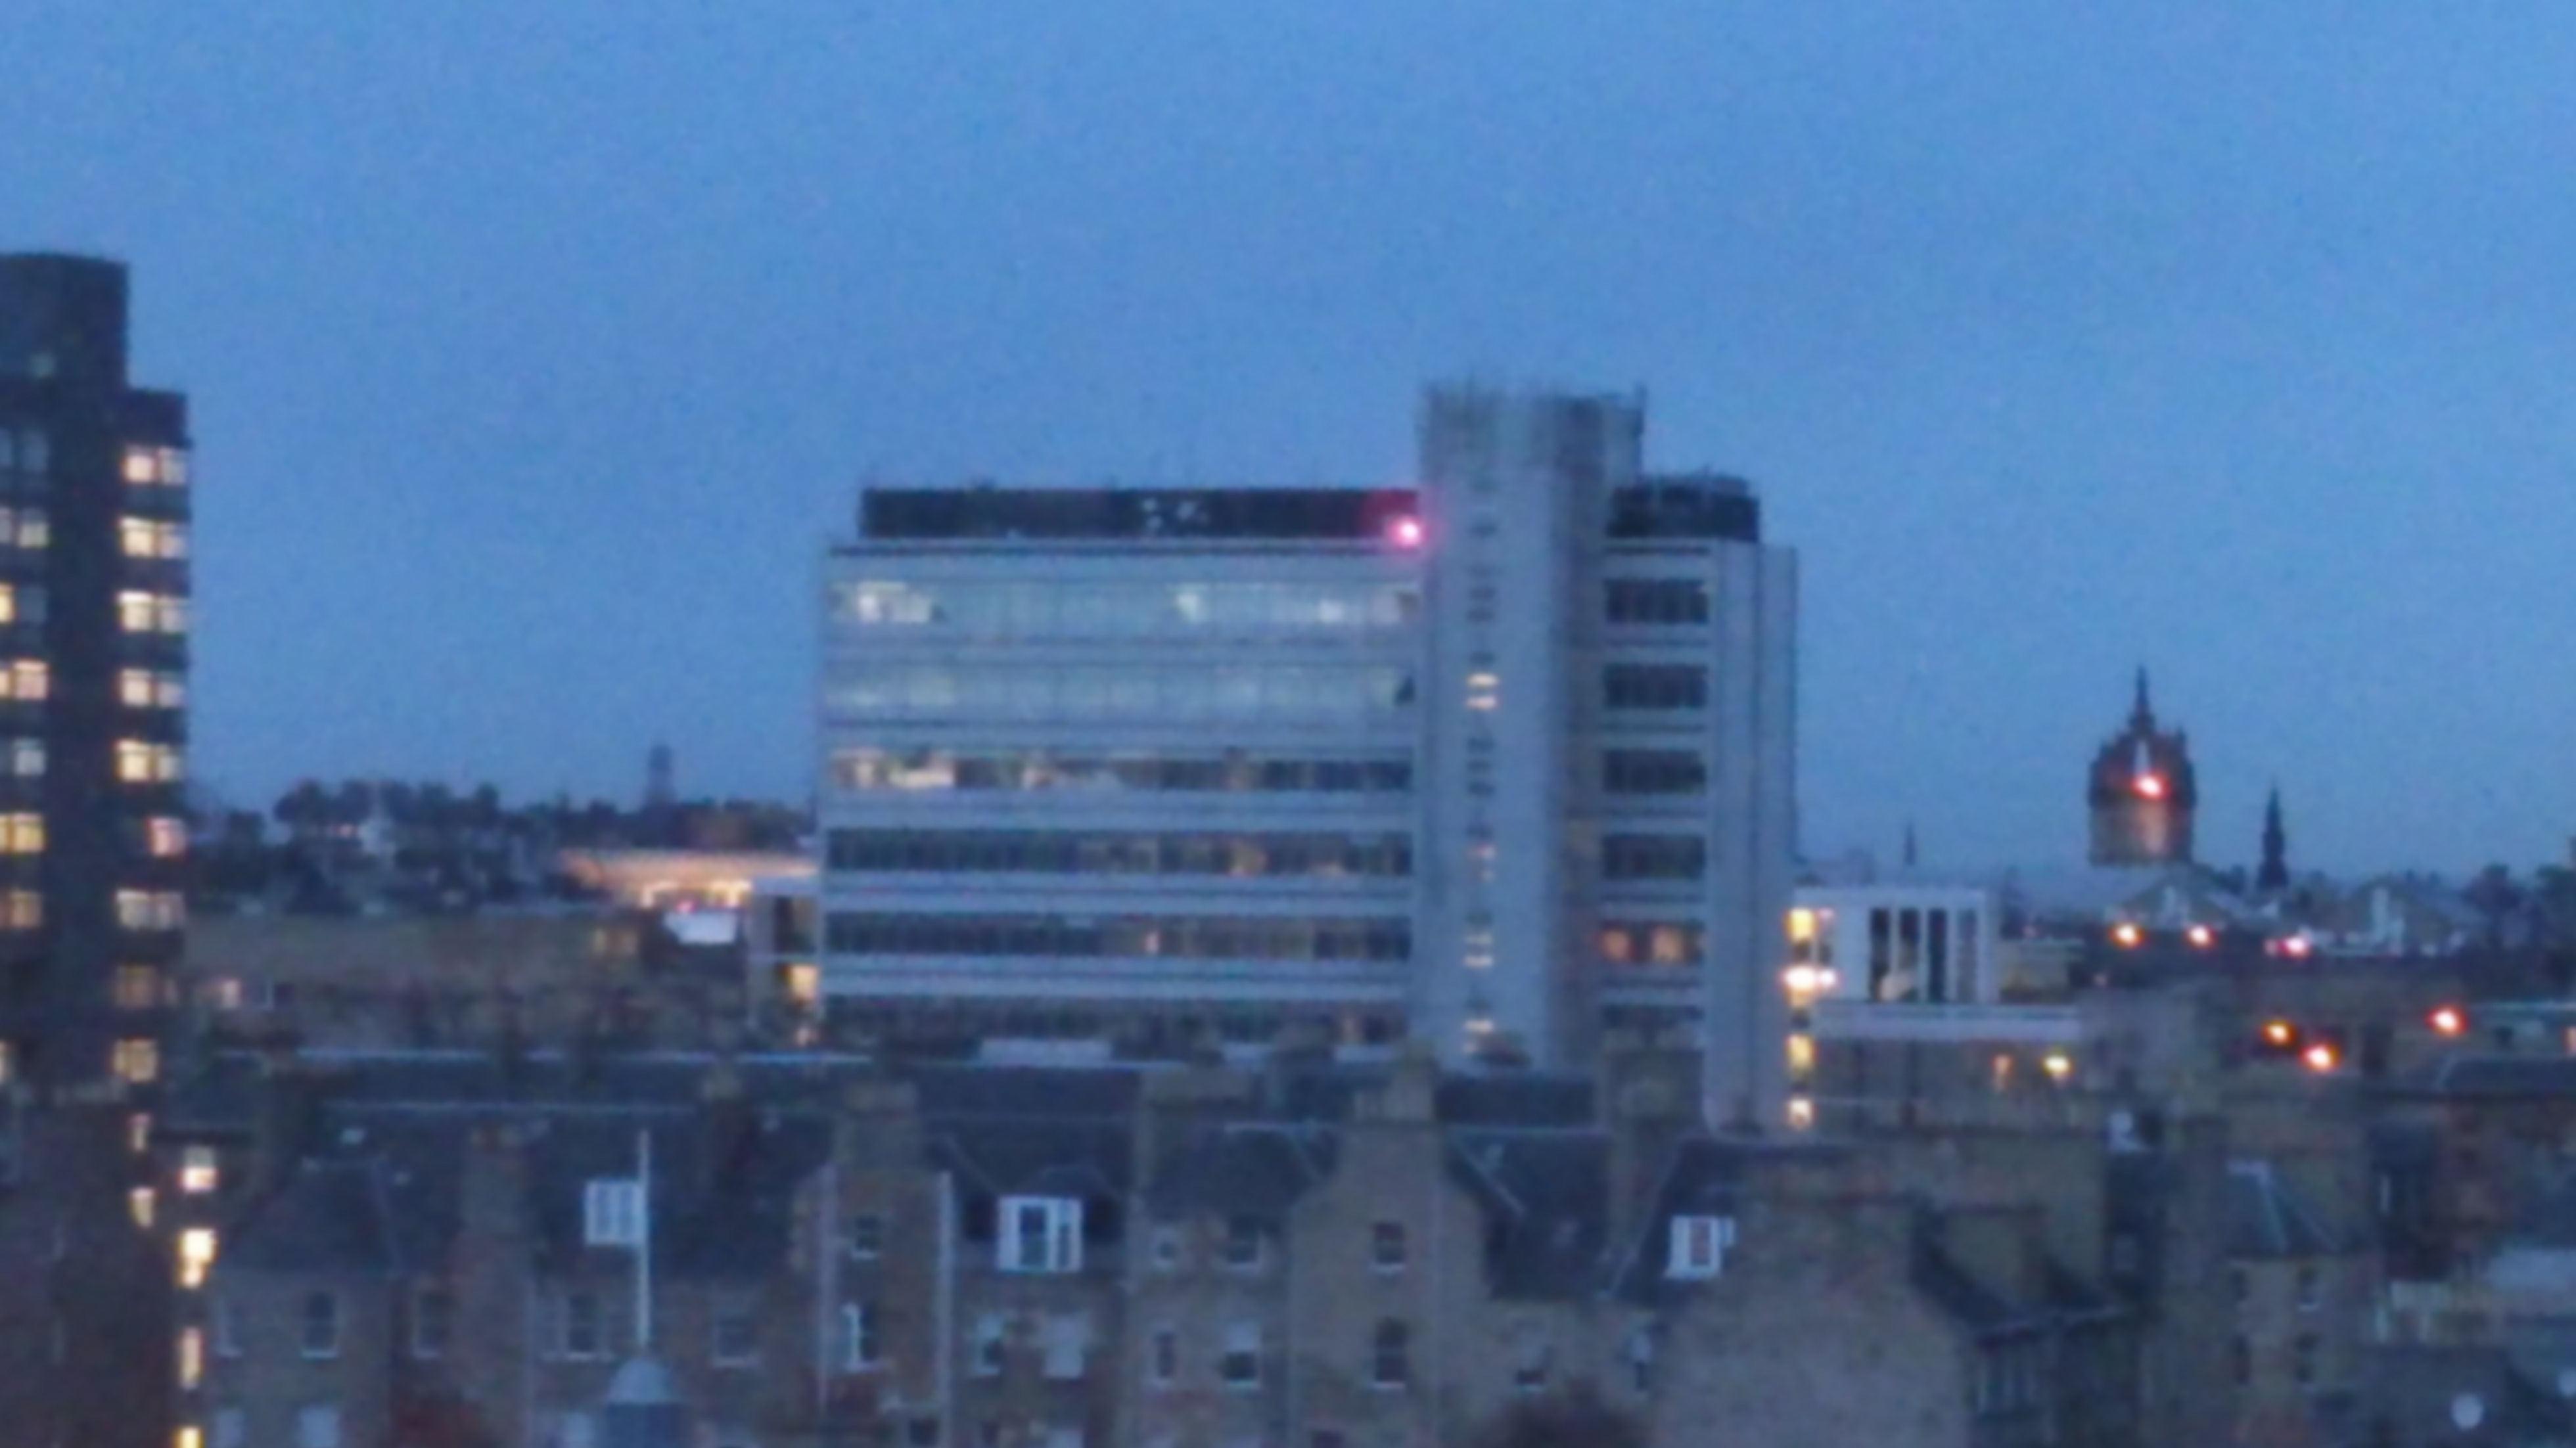
\includegraphics[width=\textwidth]{at-laser.jpg}
\end{figure}

The Scottish Government had a preferred vendor, CableFree, for the
equipment though we were formally free to select another. Our budget
was only about \pounds 10,000 for the equipment. The FSO vendors that
are well-regarded in industry such as F-Sona and Canon do not produce
anything in this price range. Small wonder as their primary market is
the military -- optical links are much harder to eavesdrop upon
compared to radio links. Two vendors were within our price range:
Geodesy of Hungary and Cablefree.

We selected the suggested vendor partly because they were a local
(i.e. UK-based) company on the theory that they might be more
responsive and accessible. We were also given to believe -- with no
evidence -- that their Hungarian competitor used inferior, older
technology. It is difficult to tell the extent to which this was
true without comparing the equipment from both manufacturers side by
side. We were subjected to the hard-sell and given very little
concrete information without signing non-disclosure agreements that
would prevent our conducting any useful research. As it was, not
executing the NDAs prevented us from properly instrumenting the
equipment and measuring its behaviour at any but very coarse
granularity.


The whole episode was without a doubt the most unpleasant interaction
with an equipment vendor in our considerable experience.

\subsection{Link Design}
\label{sec:link-design}

CableFree produced a link design as shown in
Figure~\ref{fig:cablefree-link}. In principle it is plausible,
consisting of a laser link, and a back-up radio link between Appleton
Tower and the Tech Cube, a distance of about 500m. At either end two
switches would use the spanning-tree protocol (STP) configured with the
radio link having a higher cost than the laser link. The principle
being that traffic would flow over the lasers unless they were
unavailable in which case the backup link would be used.
\def\cfdesign{%
    \node[draw,rotate=90] (atnetgear) at (0,0) {Netgear Switch};
    \node[draw] (atlaser) at (2,1) {Laser};
    \node[draw] (atradio) at (2,-1) {Radio};
    \node[draw] (tclaser) at (6,1) {Laser};
    \node[draw] (tcradio) at (6,-1) {Radio};
    \node[draw,rotate=-90] (tcnetgear) at (8,0) {Netgear Switch};
    \draw[thick,blue] (-1,0) edge (atnetgear.north);
    \draw[thick,blue] (9,0) edge (tcnetgear.north);
    \draw[thick,orange] (atnetgear.south) edge (atlaser.west);
    \draw[thick,orange] (tcnetgear.south) edge (tclaser.east);
    \draw[thick,blue] (atnetgear.south) edge (atradio.west);
    \draw[thick,blue] (tcnetgear.south) edge (tcradio.east);
    \draw[thick,red,dotted] (atlaser.east) edge (tclaser.west);
    \draw[thick,black,dotted] (atradio.east) edge (tcradio.west);
    \node at(4,0) {$\approx 500\text{m}$};
    \node at(4,1.5) {$\text{cost} = 1000$};
    \node at(4,-1.5) {$\text{cost} = 100000$};
}
\begin{figure}[h]
  \centering
  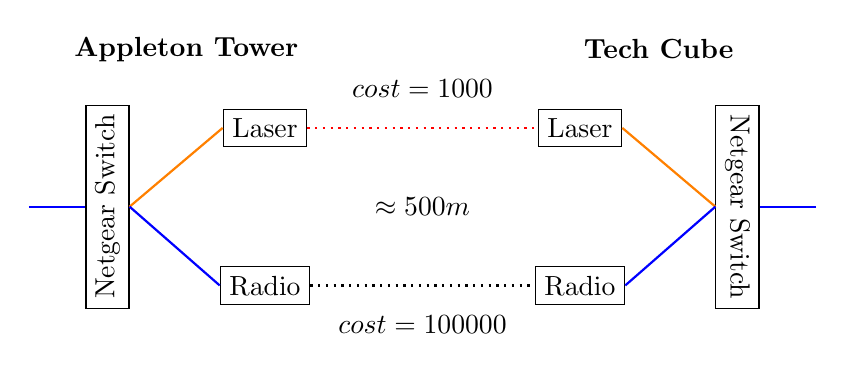
\begin{tikzpicture}
    \node at (1,2) {\textbf{Appleton Tower}};
    \node at (7,2) {\textbf{Tech Cube}};
    \cfdesign
  \end{tikzpicture}
  \caption{CableFree Link Design}
  \label{fig:cablefree-link}
\end{figure}

There were, however, several problems with this design. The less
serious was that this design was hardly appropriate for the local
environment. We already had a significant amount of radio equipment at
both sites -- including a radio link between them -- so an extra radio
link was superfluous. The radios specified by the vendor were low-end
Mikrotik radios with panel antennae in a waterproof enclosure. This is
not to cast aspersions on Mikrotik equipment, indeed we make much use
of it and it is generally quite good for the price. However Cablefree
wished to sell this re-branded equipment at a significant markup.

\begin{wrapfigure}{r}{0.3\textwidth}
  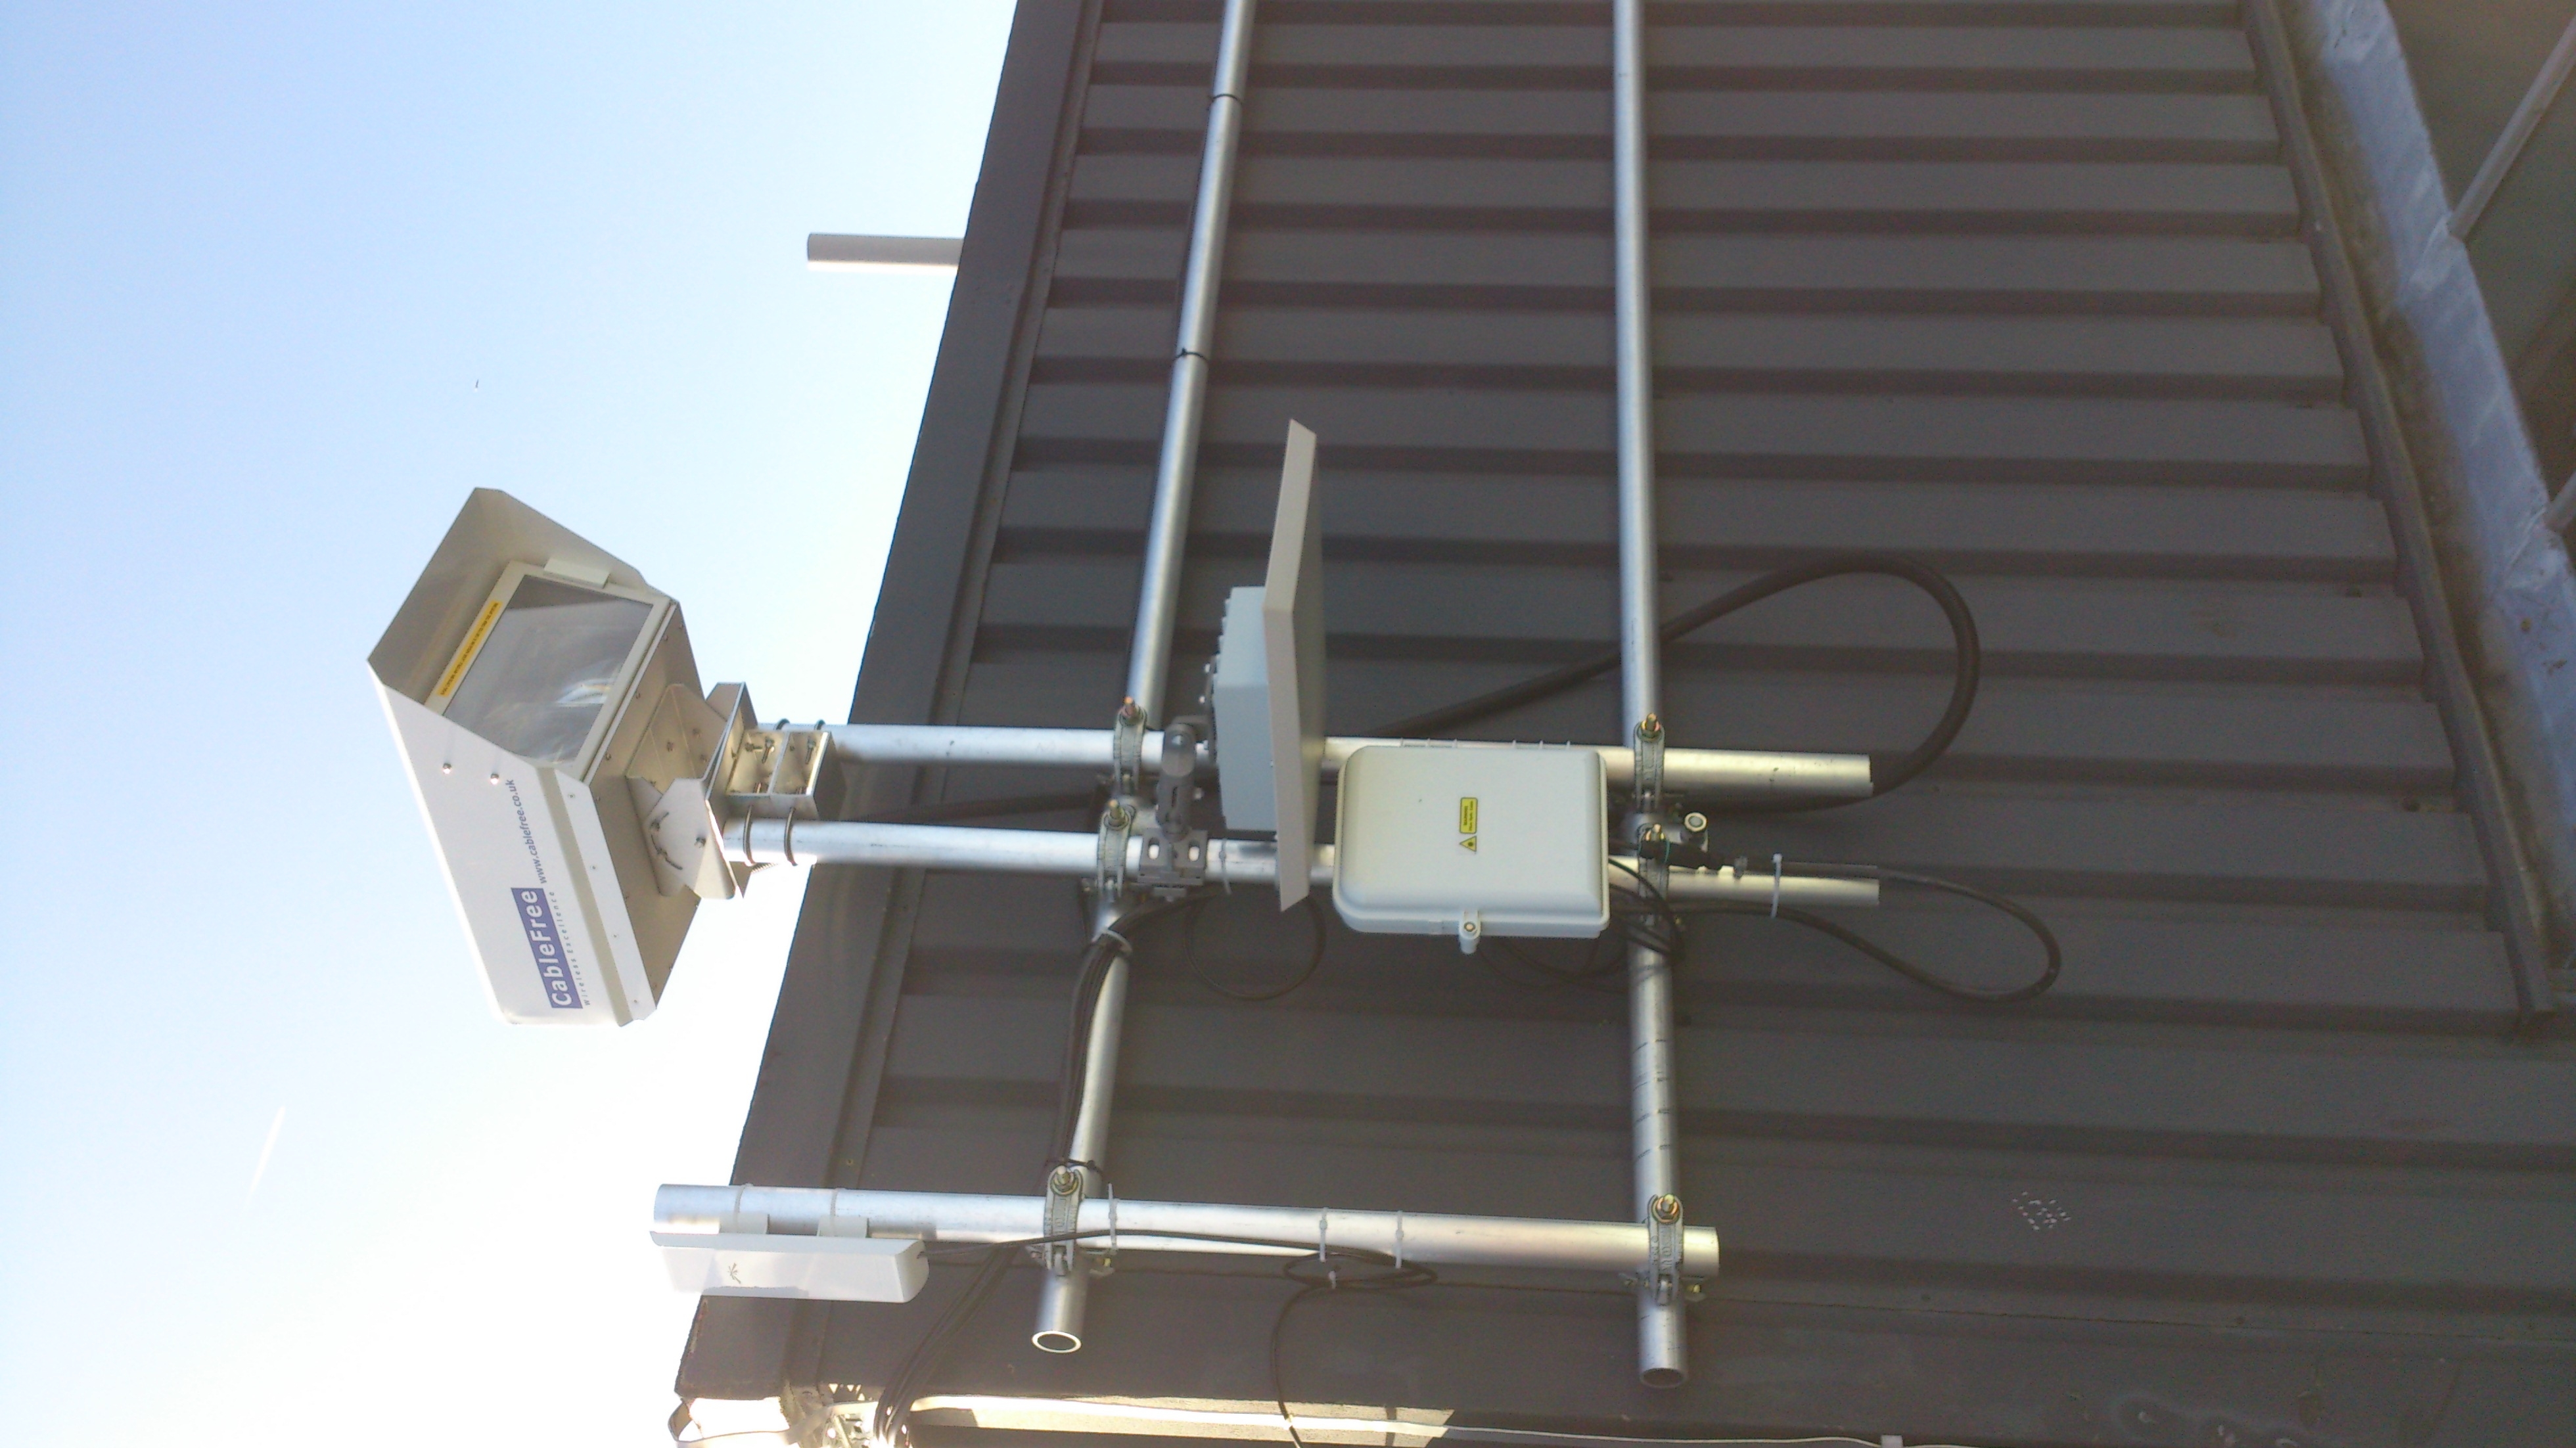
\includegraphics[angle=-90,width=0.3\textwidth]{also-faulty}
\end{wrapfigure}
Most amusingly, the mounting brackets supplied with the re-branded
Mikrotik radios were somewhat flimsy. It can get very windy at the top
of tall buildings in Edinburgh. Wind speeds can reach several times
more than at ground level. The installation is shown at right with the
mounting bracket having worked loose in high winds leaving the radio
pointing downwards.

We also had high end HP ProCurve J9050A switches at either end (loaned
by the School of Informatics), far more capable network elements than
the consumer-grade Netgear switches (see
Figure~\ref{fig:carrier-grade}) specified by the vendor. The
deficiencies of the Netgear switch are that it is not manageable via
telnet or ssh, which makes it very difficult to recover from outages
or erroneous configurations in a network of any size or complexity,
and more seriously, the cheap power adapter of the kind that are prone
to failure or simply disconnection due to the use of barrel
connectors. The power injector for the re-branded Mikrotik radio also
suffers from this deficiency (the white apparatus connected into the
switch in the photograph).

Unfortunately CableFree wished to sell a ``complete solution'' for us
to evaluate rather than an ``appropriate solution'' for our
circumstances and we succumbed to their hard-sell, ``complete'' with
sub-standard parts. We ultimately ended up operating the link by
connecting the vendor-supplied netgear switches to our HP switching
core and removing the vendor-supplied radio equipment entirely.
\begin{figure}
  \begin{center}
    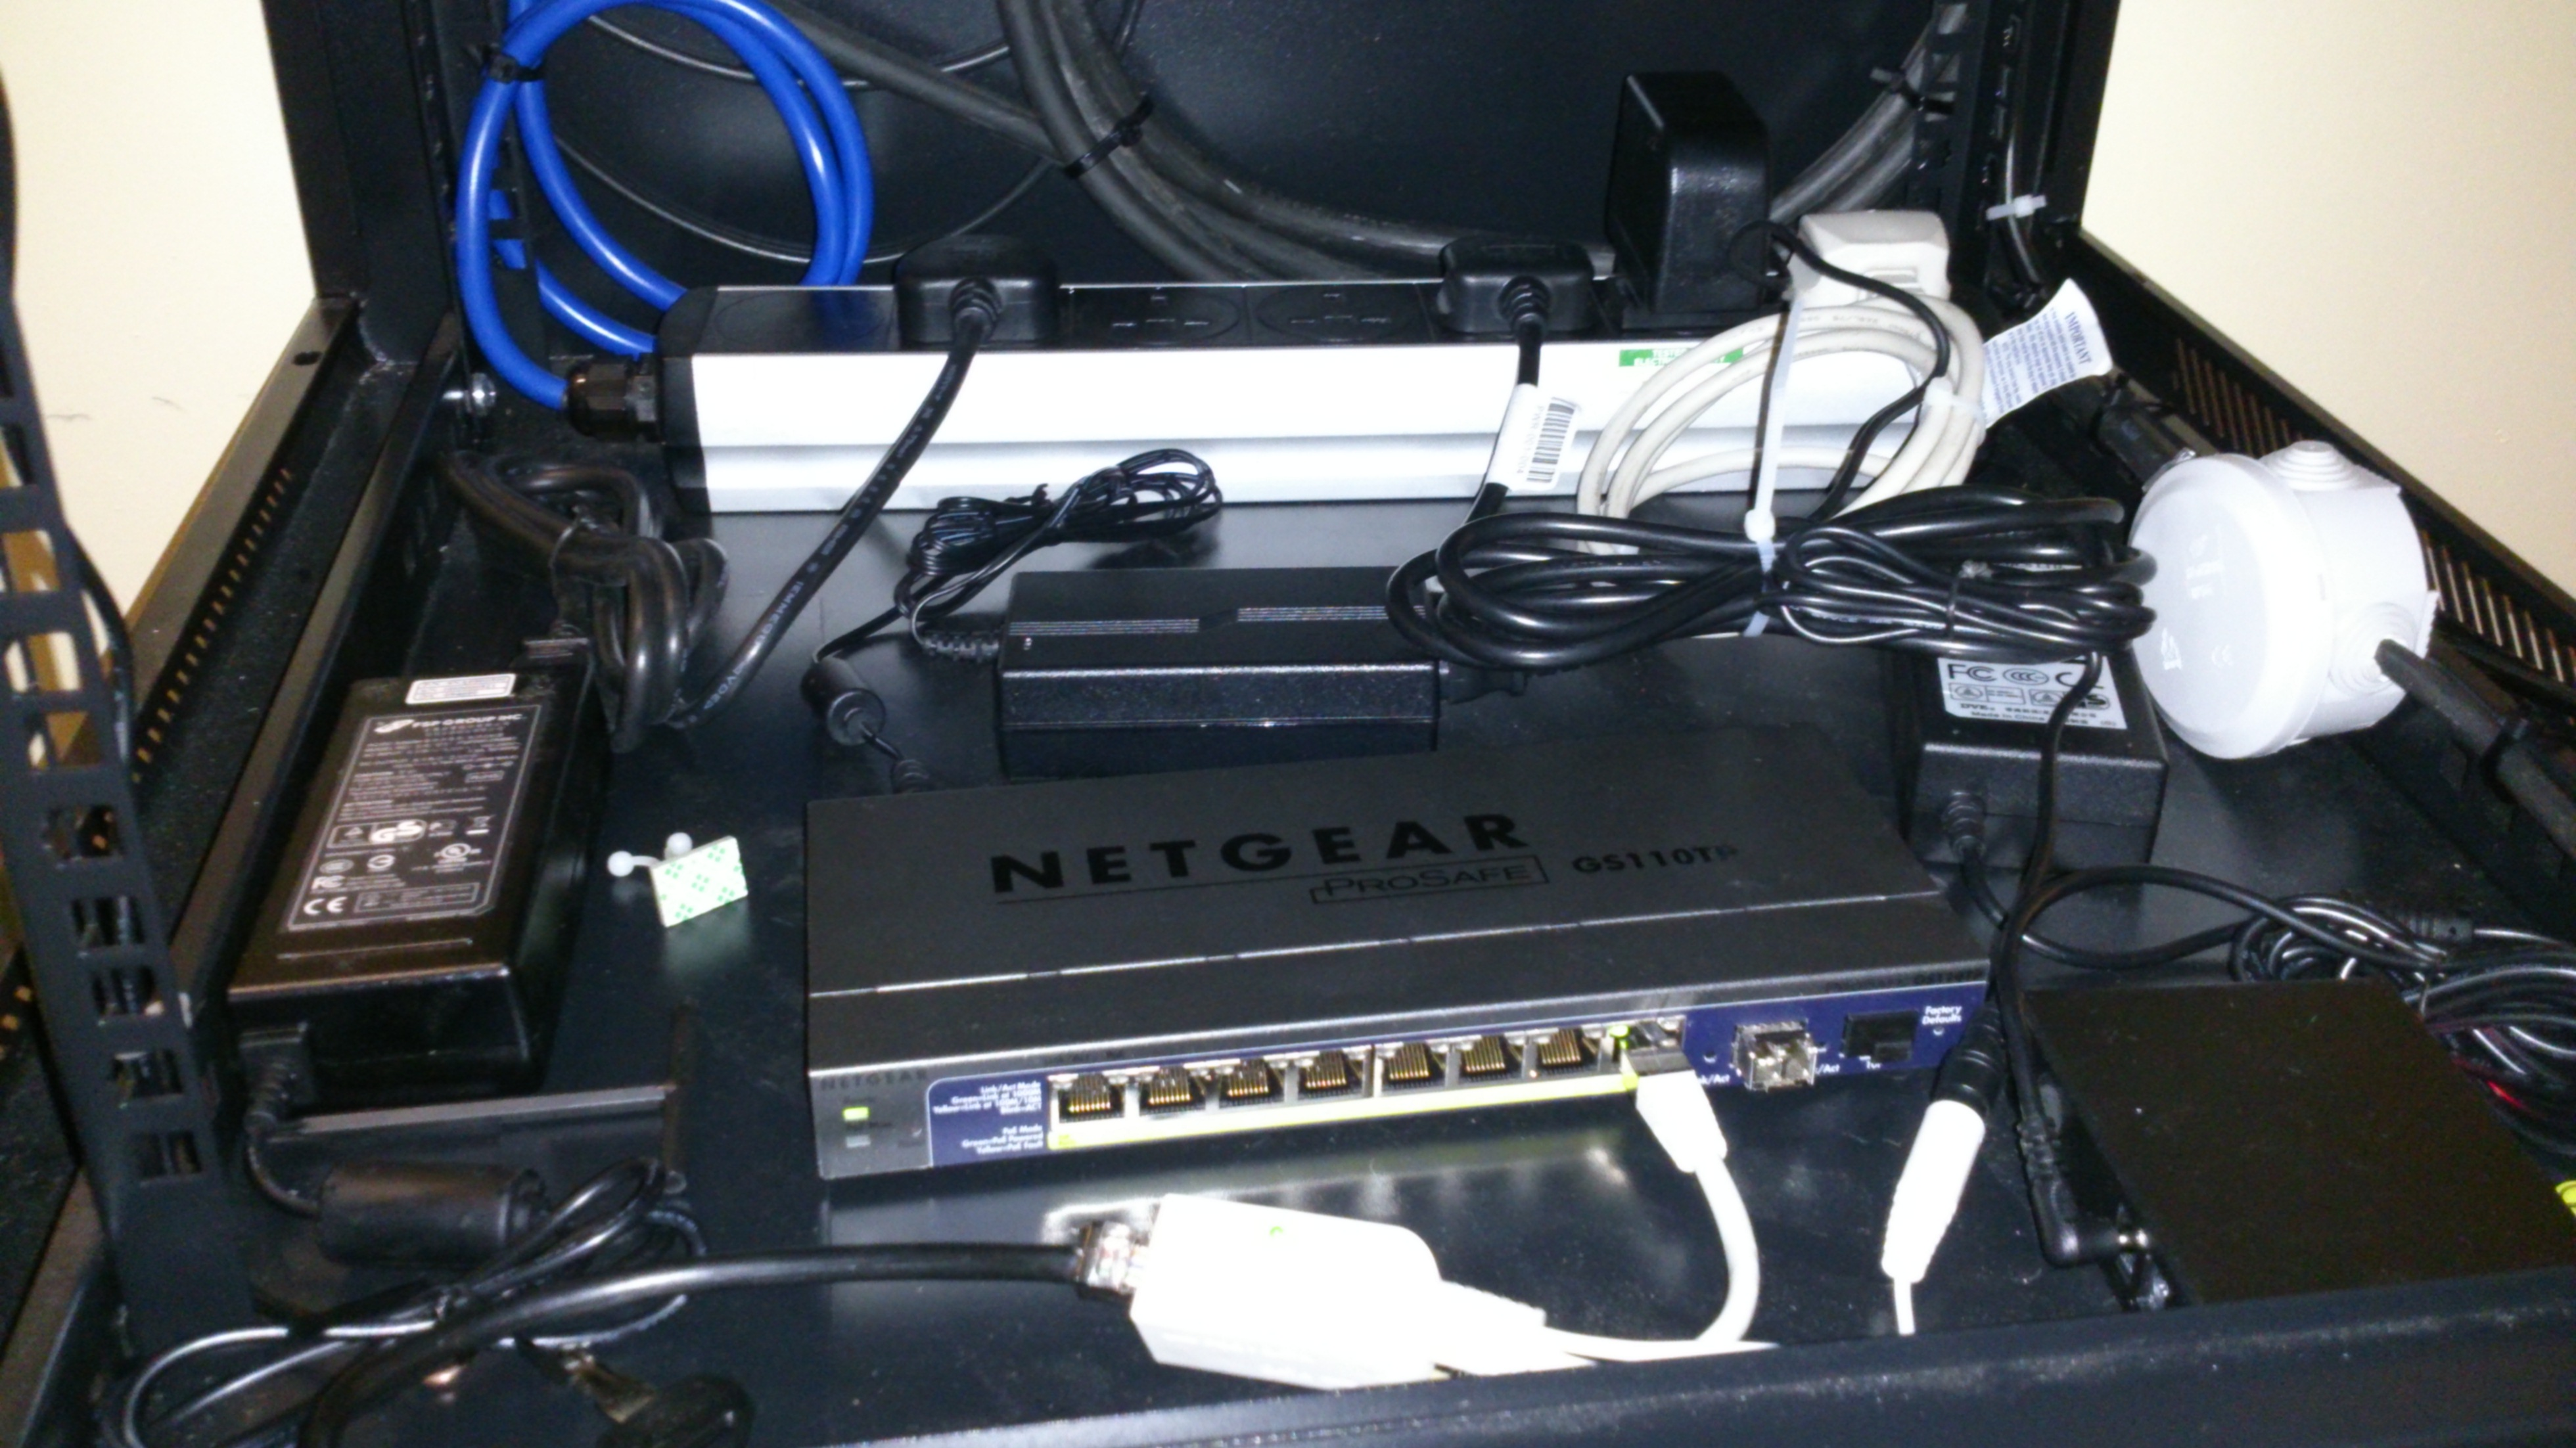
\includegraphics[width=0.5\textwidth]{carrier-grade}
  \end{center}
  \caption{A ``carrier-grade'' ethernet switch.}
  \label{fig:carrier-grade}
\end{figure}

The more serious deficiency with this design is the use of the
spanning-tree protocol. We will have more to say about the detail of
this below, but in brief, the mechanism is unstable in marginal
conditions. If the weather is clear or if the weather is very foggy,
the link operates as designed. However in the region between clear and
very foggy, the path is liable to rapidly change between the (possibly
unuseable) optical link and the radio link. Evidence for this is
anectodal due to the impossibility of properly instrumenting the
optical equipment, of which also more below.
\clearpage

\subsection{Installation}
\label{sec:fittings}

\begin{wrapfigure}{r}{0.3\textwidth}
  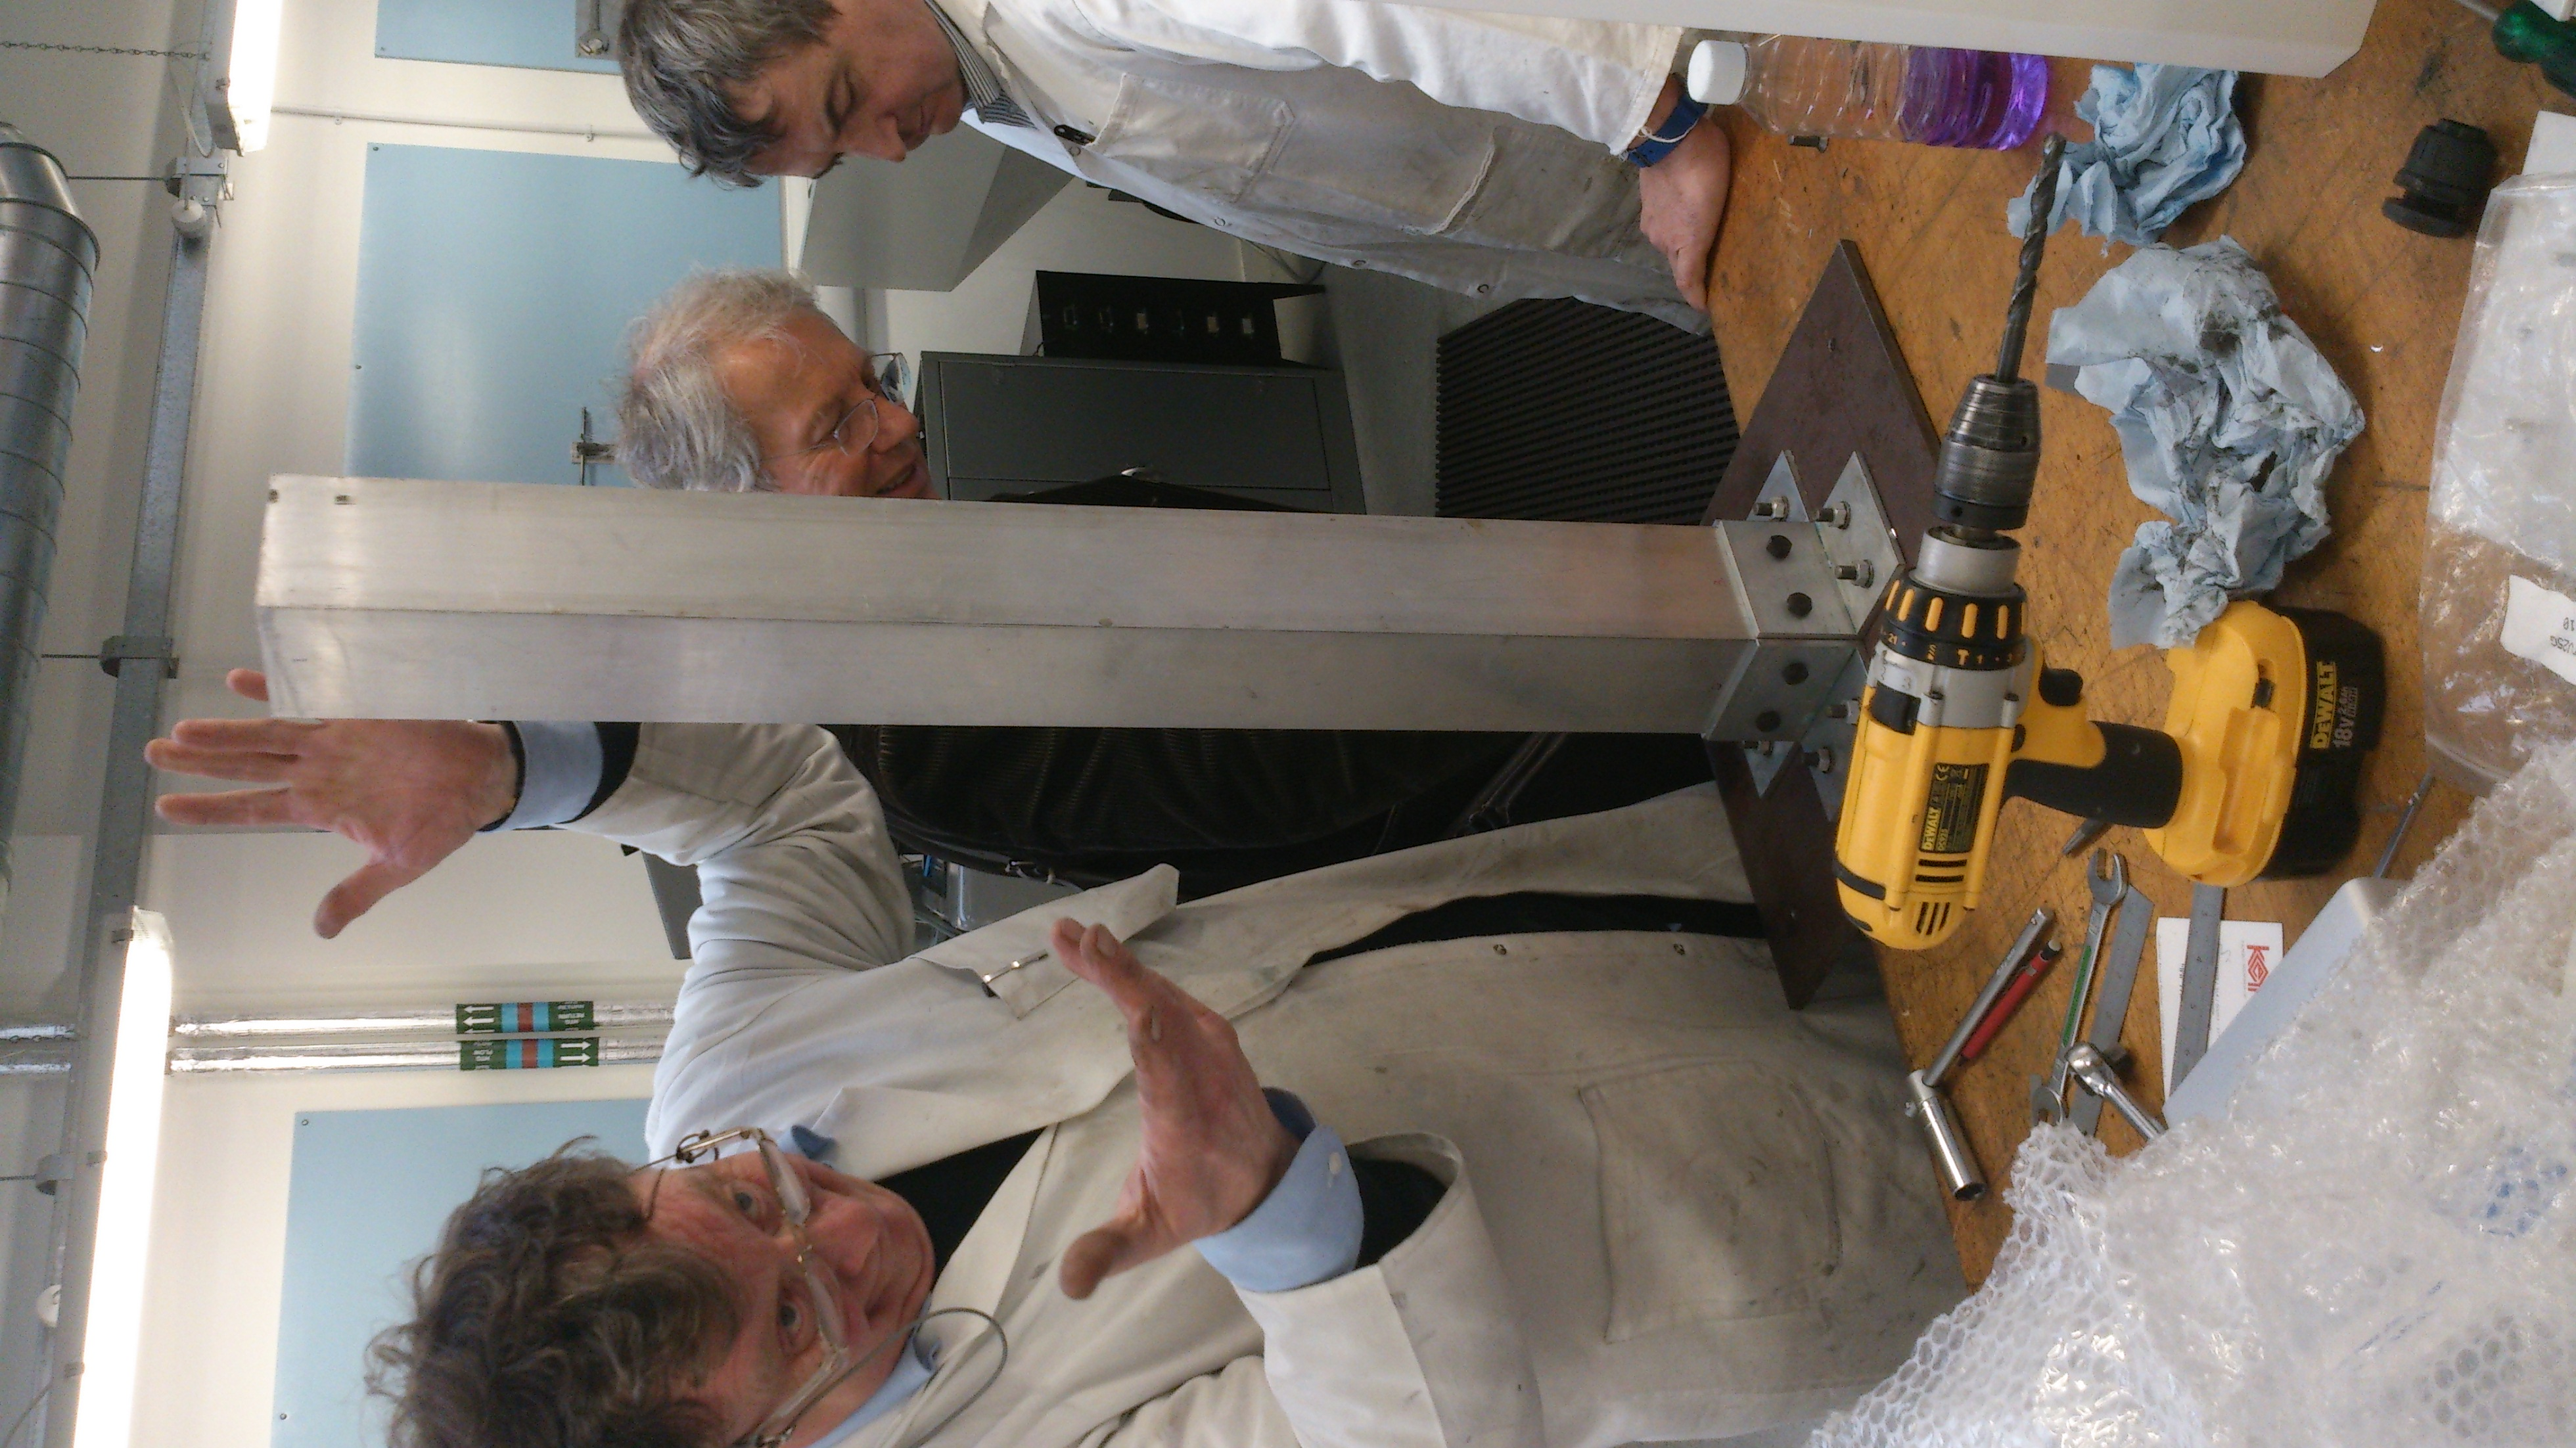
\includegraphics[angle=-90,width=0.3\textwidth]{tada}
\end{wrapfigure}
Story about trials and tribulations of getting them mounted...
The basic message from the FSO is that it works, and we have
had fewer alignment problems than I anticipated

And also how they had to have the glass screwed down because it came
off very easily...

\begin{figure}[h]
  \begin{center}
    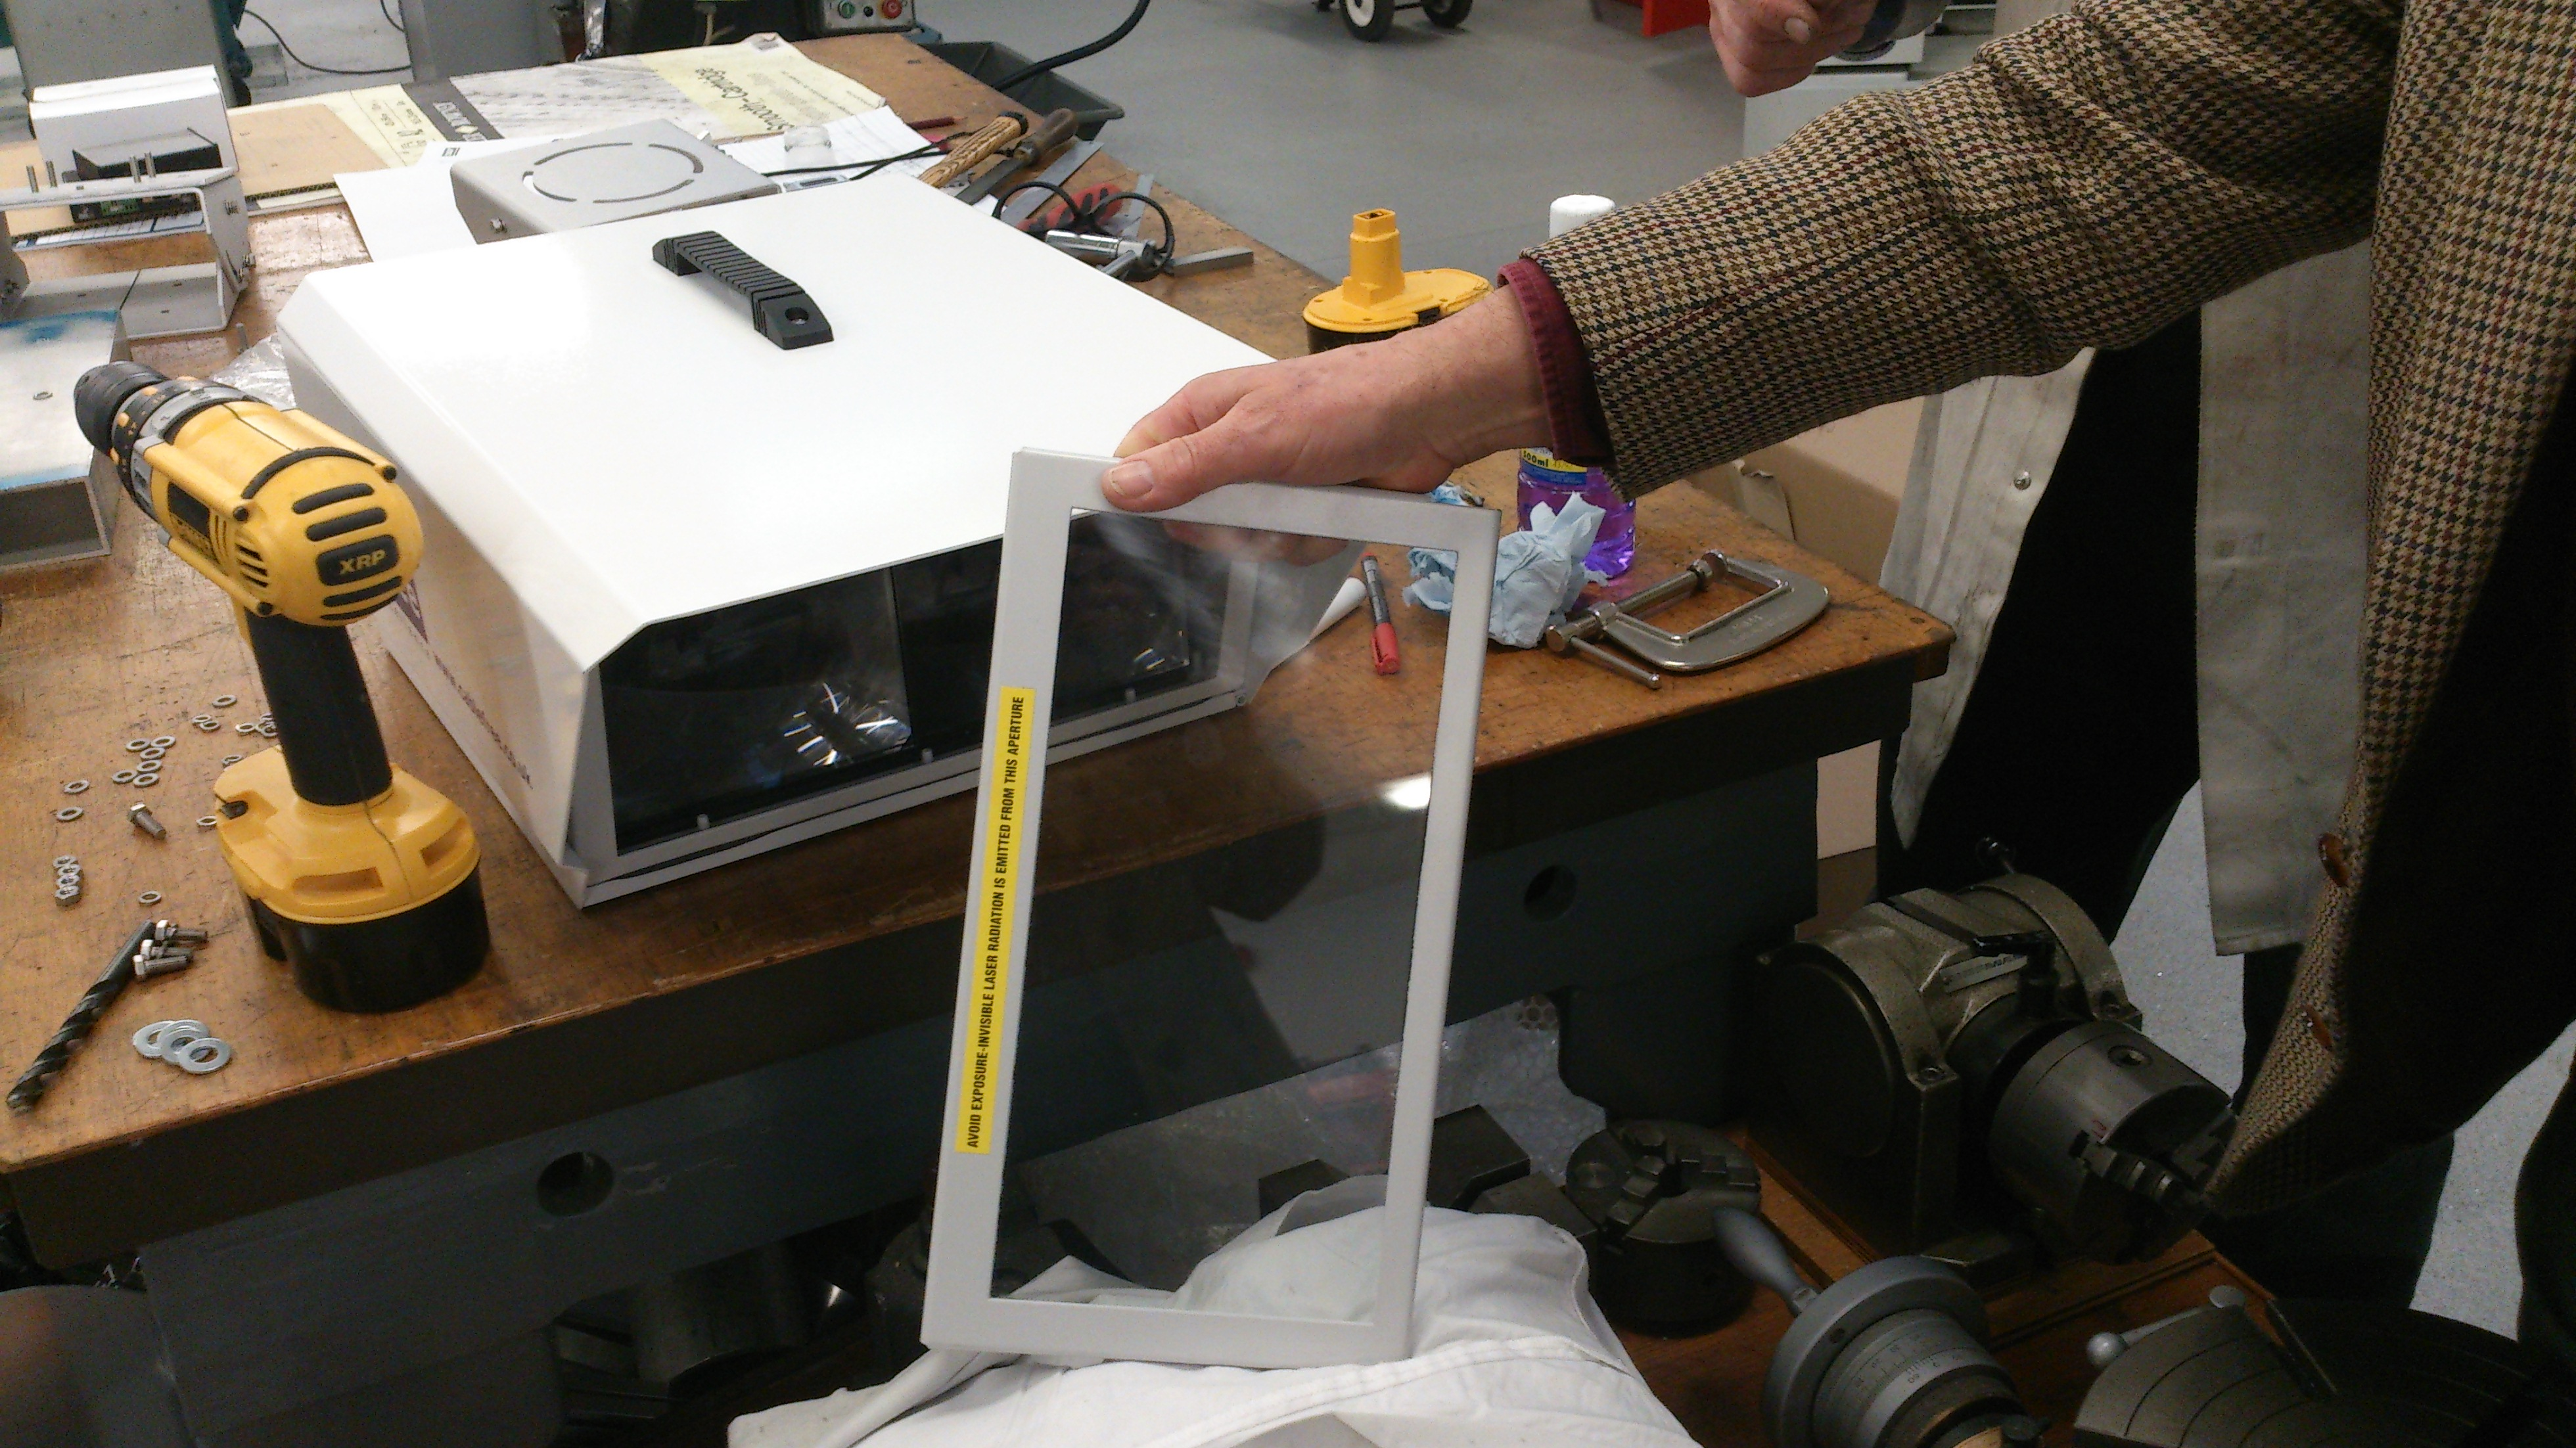
\includegraphics[width=0.5\textwidth]{faulty}
  \end{center}
\end{figure}

\clearpage
\subsection{Absorption of light by water}
\label{sec:absorption}

Unlike electromagnetic waves at radio frequencies which are not
significantly attenuated by atmospheric gasses, in the visible and
near-infrared part of the spectrum this effect plays a major role. We
all know from our experience that this is the case, for example this
effect explains why objects under water take on a blue-green tinge --
because the red part of the light reflected from them is attenuated
more by water than blue or green light. In fact we have data for this
which is shown plotted in Figure~\ref{fig:absorption-liquid} which
ranges over wavelengths from the ultraviolet (circa 380nm) to the
near-infrared (circa 800nm).
\begin{figure}[h]
  \centering
  \begin{tikzpicture}
    \begin{axis}[
      xlabel={Wavelength $\lambda$ in $\mu$m},
      ylabel={Absorption coefficient $\alpha$ in $\text{m}^{-1}$},
      xmin=0.380, xmax=0.800,
      ymin=0, ymax=3
      ]
      \node[coordinate, pin=-55:{$\alpha \approx 2.65$}]
          at (axis cs:0.380,2.65) {};
      \node[coordinate, pin=165:{$\lambda = 780\,\mu\text{m}$}]
          at (axis cs:0.780,0) {};
      \addplot[blue,thick] table {water.dat};
      \draw[red] (axis cs:0,2.65)
                    to (axis cs:0.78,2.65)
                    to (axis cs:0.78,0);
    \end{axis}
  \end{tikzpicture}
  \caption{Absorption of light by frequency through liquid water
    (\cite{jonasz_absorption_2007})}
  \label{fig:absorption-liquid}
\end{figure}

A line is marked on the diagram that shows the particular wavelength
of interest for the free-space optical equipment, 780nm. This
corresponds to an absorption coefficient of around 2.65/m$^{-1}$ which
means that through liquid water, light at this wavelength decreases in
intensity by 2.65 times for every meter of water that it travels
through.

We are not, however, intending to operate this equipment under
water. Instead we are interested in water vapour in the form of clouds
or fog, so we need to figure out how much water vapour is contained
in a given amount of air when a cloud is present. We will take cloud
formation to mean (greater than) 100\% relative humidity. This means
that the vapour pressure of water in the air is greater than the
equilibrium vapour pressure at which it evaporates and condenses at
equal rates. In fact it condenses faster than it evaporates and so the
air becomes full of condensed water droplets, or in other words a
cloud forms. The formula for this pressure commonly used in the
literature is given by~\cite{buck_new_1981} as,
\begin{equation}
  \label{eq:buck}
  e_w = (1.0007 + 3.46\times 10^{-6}P)\times 6.1121e^{\frac{17.502T}{240.97+T}}
\end{equation}
with the pressure $P$ given in hPa and the temperature in
$^\circ$C. This relation is plotted in figure~\ref{fig:water-pressure}
for a pressure of one atmosphere (1013.25 hPa).
\begin{figure}[h]
  \centering
  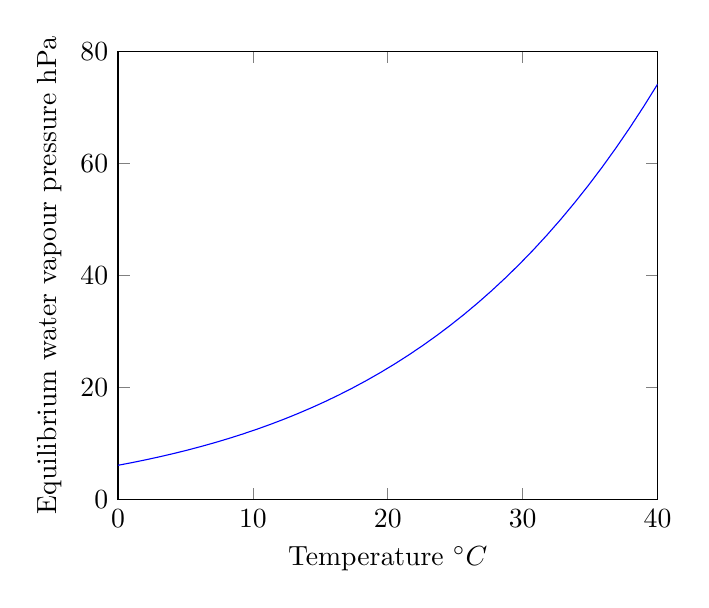
\begin{tikzpicture}
    \begin{axis}[
      ymin=0, ymax=80,
      xmin=0, xmax=40,
      xlabel={Temperature $^{\circ}\text{C}$},
      ylabel={Equilibrium water vapour pressure hPa}
      ]
      \addplot[blue,domain=0:40, samples=40]
              { (1.0007 +
                3.46e-6*1013.25)*6.1121*exp(17.502*x/(240.97+x)) };
    \end{axis}
  \end{tikzpicture}
  \caption{Water vapour density as a function of pressure}
  \label{fig:water-pressure}
\end{figure}

Since this is the minimum water vapour pressure required to form a
cloud, we may take this as a lower bound on the amount of water in the
air. At 10$^\circ$C, Buck's relation gives an equilibrium pressure of
1.23 kPa. Recalling our ideal gas law from high school,
\begin{equation}
  \label{eq:ideal-gas}
  PV = nRT
\end{equation}
we can work out that,
\begin{equation*}
  n = \frac{PV}{RT} 
    = \frac{1.23\times 10^3 \times 1}
           {8.314 \times 283}
    = 0.528\, \text{mol}
\end{equation*}
we can look up the molar mass of water, which is
18.02$\text{g}/\text{mol}$, and so arrive at a density of water in the
cloud as it is forming of 9.01$\text{g}/\text{m}^3$.

So what? Well, we know that, roughly, liquid water has a density of
1$\text{g}/\text{cm}^3$ and in terms of cubic meters this is
$10^6\text{g}/\text{m}^3$. So this tells us that we should scale the
absorption factor for water by $9.01\times 10^{-6}$ at the point of
cloud formation, which gives an adjusted absorption factor of
$2.39\times 10^{-5}$. Over the course of our 500m path, this means
that loss due to absorption (heating of the cloud) is only about
1\%.

In practice, this value is an overestimate, owing primarily to the
fact that water vapour does not behave as an ideal gas near the phase
transition from vapour to water (condensation). Experimental
measurements (\cite{whiteman_cloud_1999}) and more sophisticated
models (\cite{tampieri_size_1976,hess_optical_1998}) give values a
couple of orders of magnitude lower for the density of water in
fog. We therefore conclude that absorption is not a significant factor
in attenuation of the signal from the lasers by fog.

\subsection{Scattering of light by water}
\label{sec:scattering}
Another possible effect on the light of the lasers by water droplets
suspended in the air is scattering, as the light is reflected in
random directions by the drops. There are various models for how
scattering happens depending on the relative dimensions of the
scattering objects (e.g. water droplets) and the wavelength of the
light concerned. Where the size of the object is large with respect to
the wavelength of light, the geometric properties of the object can be
used -- treating the object essentially like a partially silvered
mirror with some part of the ray refracting and some part reflecting
according to the empirically index of refraction. If the objects are
very small with respect to the size of a wavelength, Rayleigh
scattering can be used as an approximation to the
behaviour. Unfortunately with aerosols such as fog, neither of these
techniques can be used because the water droplets are comparable to
the size of a wavelength.

The technique which remains is to explicitly model the system of many
water droplets and to calculate their effect on the light using
Maxwell's equations. This is known as the Lorenz-Mie solution. We will
not do this either but instead heuristically show that none of the
light could possibly make it through thick fog over a distance of 500
meters.

To do this, we need to find out how many water droplets there are in a
column of fog 500 meters long and 1 square meter in cross section, and
how much space they occupy on average. Then we will do a
trick. Supposing the droplets are square in cross-section, and all of
them are laid out in a thin film one droplet thick, how much area
would they occupy?
\begin{figure}[h]
  \centering
  \def\laser{
    \begin{scope}[canvas is zy plane at x=-0.6]
      \draw[black,shade] (-0.5,-0.3) rectangle (0.5,0.3);
    \end{scope}
    \begin{scope}[canvas is xy plane at z=0.5]
      \draw[black,shade] (-1.5,-0.3) rectangle (-0.6,0.3);
    \end{scope}
    \begin{scope}[canvas is zx plane at y=0.3]
      \draw[black,shade] (-0.5,-1.5) rectangle (0.5,-0.6);
    \end{scope}
    \begin{scope}[canvas is zy plane at x=-0.5]
      \fill[ball color=red] (0,0) circle[radius=0.2];
    \end{scope}
  }
  \def\laserbeam{
    \begin{scope}[canvas is xy plane at z=0]
      \pgfsetfillopacity{0.6}
      \fill[red] (-0.5,-0.2) rectangle (10,0.2);
    \end{scope}
    \begin{scope}[canvas is zy plane at x=10]
      \pgfsetfillopacity{0.6}
      \fill[ball color=red] (0,0) circle[radius=0.2];
    \end{scope}
  }
  \begin{tikzpicture}
    \tikzset{facestyle/.style={draw=gray,very thin,line join=round}}
    \laser\laserbeam
    \begin{scope}[canvas is xy plane at z=-0.5]
      \pgfsetfillopacity{0.5}
      \path[facestyle,shade] (0,-0.5) rectangle (10,0.5);
    \end{scope}
    \begin{scope}[canvas is xy plane at z=0.5]
      \pgfsetfillopacity{0.5}
      \path[facestyle,shade] (0,-0.5) rectangle (10,0.5);
    \end{scope}
    \begin{scope}[canvas is zx plane at y=-0.5]
      \pgfsetfillopacity{0.5}
      \path[facestyle,shade] (-0.5,0) rectangle (0.5,10);
    \end{scope}
    \begin{scope}[canvas is zx plane at y=0.5]
      \pgfsetfillopacity{0.5}
      \path[facestyle,shade] (-0.5,0) rectangle (0.5,10);
    \end{scope}
    %% labels
    \begin{scope}[canvas is xy plane at z=-0.5]
      \node (d) at (5,1) {500m};
      \draw (d) edge[->] (0,1);
      \draw (d) edge[->] (10,1);
      \node at (11,0) { 1m };
      \draw (10.5,-0.5) edge[<->] (10.5,0.5);
    \end{scope}
  \end{tikzpicture}
  \par\vspace{\baselineskip}
  \begin{tikzpicture}
    \tikzset{facestyle/.style={draw=gray,very thin,line join=round}}
    \laser
    \begin{scope}[canvas is xy plane at z=0]
      \pgfsetfillopacity{0.6}
      \fill[red] (-0.5,-0.2) rectangle (1,0.2);
    \end{scope}
    \begin{scope}[canvas is xy plane at z=0]
      \draw[red] (1,0.2) edge[->] (0,1);
      \draw[red] (1,-0.2) edge[->] (0,-1);
    \end{scope}
    \begin{scope}[canvas is zy plane at x=1]
      \pgfsetfillopacity{0.6}
      \fill[ball color=red] (0,0) circle[radius=0.2];
      \draw[teal,fill=teal] (-0.707,-0.707) rectangle (0.707,0.707);
    \end{scope}
  \end{tikzpicture}
  \caption{Top: a 500m column of fog. Bottom: scattering off of a
    reflective thin film of droplets.}
  \label{fig:column-fog}
\end{figure}
The calculation isn't difficult, we just need the average radius of a
droplet which we will take from~\cite{hess_optical_1998} for a dense
fog, $10.7\,\mu\text{m}$, and the density of water in such a fog from
the same source, $0.058\,\text{g}/\text{m}^3$. 
\begin{align}
  \rho_{\text{l}} &&=&\quad 10^6\,\text{g}/\text{m}^3 
  &\qquad\text{Density of liquid water}\\
  \rho_{\text{f}} &&=&\quad 0.058\,\text{g}/\text{m}^3
  &\qquad\text{Density of fog}\\
  V_d &= \frac{4}{3}\pi r^3 &=&\quad 5.13\times 10^{-13}\,\text{m}^3
  &\qquad\text{Volume of a water droplet}\\ 
  m_d &= \rho_{\text{l}} V_d &=&\quad 5.13\times 10^{-7}\,\text{g}
  &\qquad\text{Weight of a water droplet}\\
  n &= \rho_{\text{f}}/m_d &=&\quad 1.13\times 10^{7}
  &\qquad\text{Number of droplets per unit volume}\\
  N &= 500n &=&\quad 5.65\times 10^{9}
  &\qquad\text{Number of droplets in a 500m column}\\
  a_d &= \pi r^2 &=&\quad 3.597\times 10^{-10}\,\text{m}^2
  &\qquad \text{Cross-sectional area of a droplet}\\
  A &= Na_d &=&\quad 2.03\,\text{m}^2
  &\qquad \text{Surface area of thin film}
\end{align}

This shows that with evenly distributed thick fog it can be expected
that a given ray of light will meet at least two droplets -- and hence
certainly be scattered -- in a distance of 500m. Alternatively we only
need a path of 250m to be sure that all of the light from the laser
will be scattered. We can therefore be satisfied that such optical
links will not function in the presence of fog.

\clearpage
\subsection{Instrumentation}

\subsection{Correlation of link operation with weather}
\label{sec:weather}

We have been monitoring availability of the optical link and I have
access to the UK hourly weather data for the purposes of this project
(1.4 GB for 2014, so far only 79 MB for 2014, which is just
January). Unfortunately we had to undertake some emergency works in
November to make way for Vodaphone at Summerhall, and it turns out
that this has interfered with some of our data-collection.

(Analysis here)

%%% Local Variables:
%%% mode: latex
%%% TeX-master: "scotgov-report"
%%% reftex-default-bibliography: ("literature.bib")
%%% zotero-collection: #("28" 0 2 (name "Papers/Scotgov Report"))
%%% End:
